% PAKETE UND DOKUMENTKONFIGURATION
\documentclass[10pt, a4paper]{article}

% Encoding für Umlaute
\usepackage[utf8]{inputenc}

% Silbentrennung
\usepackage[ngerman]{babel}

% erweiterte Matheumgebungen
\usepackage{amsmath}

%
\usepackage{amsfonts}

%
\usepackage{amssymb}

% Einheiten setzen z.B. \SI{10}{\kilo\gram\meter\per\second\squared}
% Fehler: \SI{10 +- 0,2e-4}{\metre}
\usepackage{siunitx}
\sisetup{
  output-decimal-marker={,},
  separate-uncertainty
}

% Randbreiten
\usepackage[left=3cm,right=4cm,top=3cm,bottom=3cm,twoside]{geometry}

% Bilder einfügen
\usepackage{graphicx}

%Verwise innerhalb des Dokuments
\usepackage{hyperref}
\hypersetup{
	colorlinks = true,
	allcolors = {black}
}

% Tiefe des Inhaltsverzeichnisses (Level: 1 sections, 2 subsections,
% 3 subsubsections)
\setcounter{tocdepth}{2}

% DOKUMENTINFORMATIONEN
\title{P422 \\ Rastertunnelmikroskopie}

\author{Christopher Deutsch\footnote{christopher.deutsch@uni-bonn.de} \and Christian Bespin\footnote{christian.bespin@uni-bonn.de}}

\date{\today}

\begin{document}
  
\maketitle

% DURCHFÜHRUNGSDATUM UND ASSISTENT
\begin{center}
\begin{tabular}{l r}
Durchführung: & 20./21. Oktober 2014 \\
Gruppe: & 2 $\alpha$ \\
Assistent: & Peter Klassen
\end{tabular}
\end{center}

% ZUSAMMENFASSUNG
\begin{abstract}
% Text
\end{abstract}

% INHALTSVERZEICHNIS
\tableofcontents
% Neue Seite nach TOC
\newpage

% INHALT VERSUCHSPROTOKOLL
\section{Grundlagen}

\subsection{Tunneleffekt und Tunnelstrom}
Der Tunneleffekt ist ein quantenmechanisches Phänomen, welches einem einlaufenden Teilchen der Energie $E$ erlaubt, eine klassisch unüberwindbare Potentialschwelle der Höhe $V_0 > E$ mit endlicher Wahrscheinlichkeit zu durchqueren.
Im Gegensatz zum klassischen Fall, bei dem das Teilchen am Potentialwall reflektiert wird, nimmt bei der quantenmechanischen Beschreibung das Betragsquadrat der Wellenfunktion $|\Psi|^2$ und damit die Aufenthaltswahrscheinlichkeitdichte des Teilchens, exponentiell mit der Eindringtiefe $s$ ab.

Dieser Effekt wird beim Rastertunnelmikroskop (RTM) ausgenutzt, indem eine Spannung zwischen dem zu untersuchenden, leitenden Objekt und der ebenfalls leitenden Spitze des RTM angelegt wird. Dadurch können Elektronen aus der Probe in die Spitze tunneln (oder umgekehrt), was zu einem Stromfluss $I_T$ führt.
Der Tunnelstrom für eine Potentialschwelle der mittleren Höhe $\Phi$ (für kleine Vorspannungen $U$ ist dies gegeben durch die Austrittsarbeit der Probe \cite{colton}) ist gegeben durch \cite{binning}:
\begin{equation}
  I_T \propto \exp(-\alpha \cdot \sqrt{\Phi} \cdot s) \quad \text{mit}\: \alpha = \SI{1,025}{\angstrom^{-1}\electronvolt^{-1/2}}
  \label{eq:tunnelstrom}
\end{equation}
also abhängig vom Abstand Spitze-Probe $s$, sowie von deren elektronischen Eigenschaften.
An Gleichung \ref{eq:tunnelstrom} erkennt man bereits die hohe Sensitivität auf Abstandsänderungen in der Größenordnung von einem \si{\angstrom}.
Aus diesem Grund ist das letzte Atom auf der Spitze maßgeblich für den gemessenen Tunnelstrom.

\subsection{Funktionsweise des Rastertunnelmikroskops}
\subsubsection{Aufbau}
\begin{figure}[h]
\centering
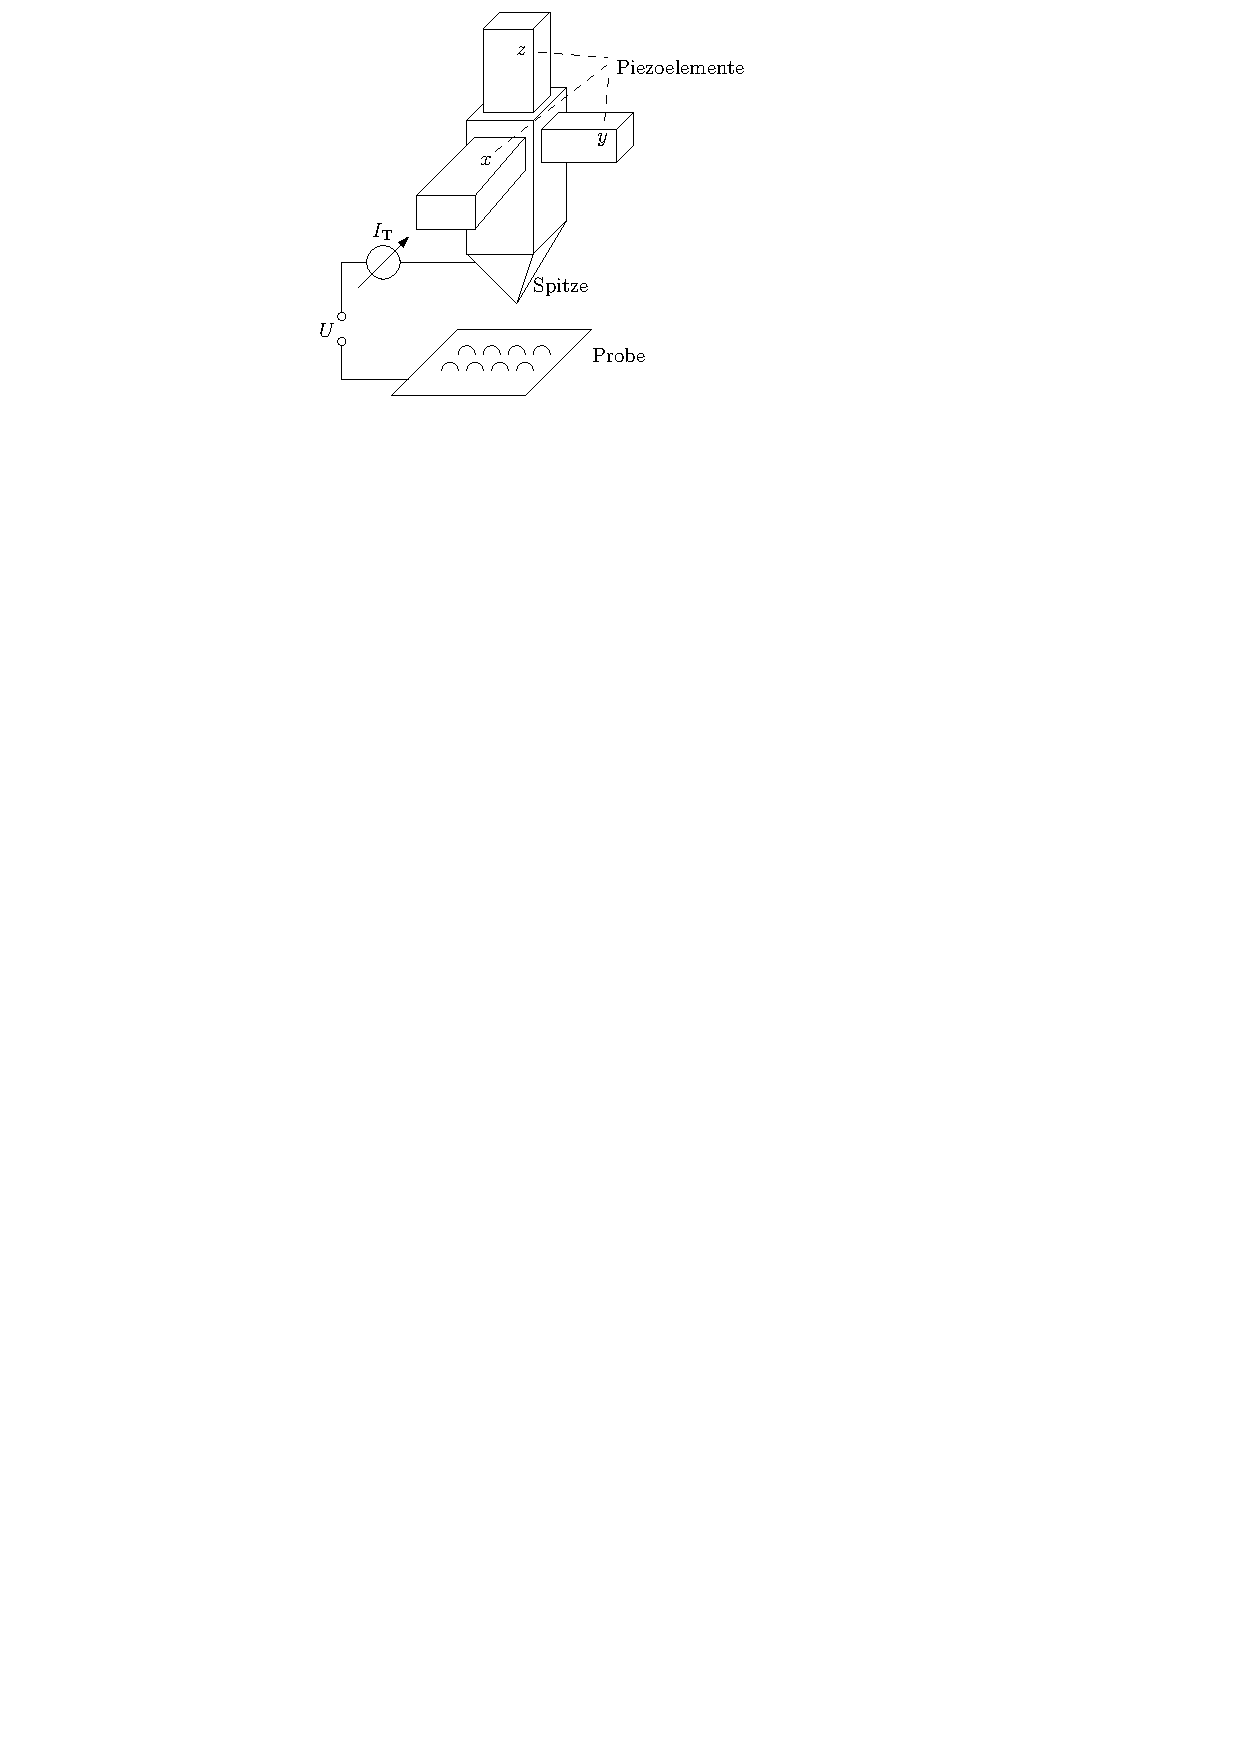
\includegraphics[width=0.5\textwidth]{./grafiken/rtm_aufbau.pdf}
\caption{schematischer Aufbau eines RTM mit Piezoelementen}
\label{fig:aufbau}
\end{figure}
Abbildung \ref{fig:aufbau} zeigt den schematischen Aufbau eines Rastertunnelmikroskops.
Dabei wird der Tunnelstrom $I_T$ gemessen und je nach Betriebsmodus (s.u.)  ausgewertet.
Die Piezoelemente dienen der Bewegung der Spitze in alle drei Raumrichtungen, wobei sie entweder automatisch gesteuert werden können (s. konstanter Tunnelstrom unter \ref{sec:betriebsmodi}) oder direkt gesteuert werden können zur manuellen Ausrichtung der Spitze.
\begin{itemize}
  \item Subatomare Auflösung -- Piezoeffekt
\end{itemize}
\subsubsection{Piezoeffekt}
In Elementarzellen mit nicht-inversionssymmetrischer Ladungsverteilung kann, beim Anlegen eines externen elektrischen Feldes, ein elektrisches Dipolmoment induziert werden.
Diese Polarisation führt zu einer Längenkontraktion/-ausdehnung der Elementarzelle aufgrund der Asymmetrie der Ladungsverteilung.
Dieser Effekt wird makroskopisch als Längenänderung eines piezoelektrischen Zylinders bei angelegter Spannung sichtbar.

\subsubsection{Betriebsmodi}
\label{sec:betriebsmodi}
Wir gehen im Folgenden davon aus, dass wir die Spannung zwischen Spitze und Probe in beiden Fällen konstant lassen.
Dann sind im Betrieb eines Rastertunnelmikroskops grundsätzlich zwei Betriebsmodi zu unterscheiden:
einmal wird der Tunnelstrom konstant gehalten, während im anderen Fall die Höhe der Spitze über der Probe konstant gehalten wird.
Im Fall des konstanten Tunnelstroms folgt die Spitze dem Profil der Probe.
Dies wird erreicht, indem der Tunnelstrom gemessen wird und durch eine Rückkopplungsschleife die Spitze so positioniert wird, dass der Tunnelstrom einen konstanten, vorgegebenen Wert annimmt.
Dafür sind die Piezoelemente notwendig, deren angelegte Spannung durch einen Regelkreis gesteuert wird.
Dessen Reaktionszeit sorgt dafür, dass das Verfahren im Vergleich zum Betriebsmodus mit konstanter Höhe deutlich langsamer ist, jedoch wird hier die Gefahr eines Zusammenstoßes von Spitze und Probe  unterbunden.

Im zweiten Fall wird die Spitze mit einer festgelegten und konstanten Höhe über die Probe bewegt und der Tunnelstrom gemessen.
Da seine Abhängigkeit von der elektronischen Struktur der Probe bekannt ist, lässt sich so ein Bild der Probe erstellen.
Da außer der Bewegung der Spitze in einer Ebene keine weiteren Regelungen notwendig sind, ist dieses Verfahren geeignet, um in kurzer Zeit Bilder der Probe zu erhalten, allerdings besteht dabei die Gefahr einer Kollision, bei dem die Spitze in die Probe fährt und dadurch zerstört wird.
Dieser Betriebsmodus ist also für flache Strukturen der Probe mit einer durchschnittlichen Höhe kleiner als der Abstand Probe-Spitze geeignet \cite{colton}.
Da es praktisch kaum möglich ist, vertikale Verschiebungen auszuschließen und die Probe nicht immer parallel zur horizontalen Bewegung der Spitze ausgerichtet ist, wird auch hier eine Rückkopplungsschleife, wie oben erklärt, verwendet, allerdings mit einer geringen Empfindlichkeit. Dadurch ist sichergestellt, dass die Spitze nicht auf schnelle Änderungen des Tunnelstroms reagiert, aber langfristig eine vorgegebene Höhe über der Probe (auch wenn diese gegen die horizontale Bewegungsebene der Spitze geneigt ist) erreicht wird.
 
\begin{itemize}
  \item Konstanter Tunnelstrom (Rückkopplungsschleife und deren Reaktionszeit, proportional zum Probenprofil)
  \item Konstante Höhe (Tunnelstrom wird aufgezeichnet, proportional zur elektronischen Struktur, \emph{Crash}, schnell)
\end{itemize}

\subsubsection{Regelkreis}

Wie oben angesprochen, dient der Regelkreis dazu, den Tunnelstrom konstant zu halten.
Dafür wird dieser kontinuierlich gemessen und entsprechend seines aktuellen Wertes wird das Piezoelement zur Höhensteuerung der Spitze mit einer Spannung versorgt, damit der Tunnelstrom einen vorgegebenen Wert annimmt.
Da $I_T$ exponentiell von der Höhe abhängt (und weiteren Faktoren), wird der Tunnelstrom zunächst logarithmiert, um ein direkt von der Höhe $s$ der Spitze über der Probe proportionales Signal zu erhalten.
Daraus kann dann die Höhe ermittelt werden und der Tunnelstrom über eine Rückkopplung auf einen vorgegebenen Wert eingestellt werden. 
Dies geschieht durch eine entsprechende Spannung an den Piezoelementen, die die Höhe der Spitze über der Probe kontrollieren.

Es gibt verschiedene Reglertypen, deren Unterscheidung grundsätzlich nach ihrer Art, zu schalten, erfolgt.
So genannte P-Regler liefern beispielsweise ein zur Eingangsgröße proportionales Signal mit einer festen Verstärkung und schalten sprunghaft.
In der Praxis werden solche Regler meist um eine integrierende und/oder differenzierende Funktion erweitert. Entsprechend spricht man dann beispielsweise von PI- oder PID-Reglern.
Der integrierende Teil sorgt für eine zeitabhängige Schaltung, so dass auch die Eingangsgröße eine gewisse Zeit in der Vergangenheit überwacht wird und daraufhin ein entsprechendes Schaltverhalten eintritt, welches dann auch nicht sprunghaft, sondern linear abläuft.
Der differenzierende Teil hingegen reagiert nicht auf den Wert des Eingangssignals sondern auf seine Änderungsgeschwindigkeit.
Auf einen linearen Anstieg am Eingang folgt dann beispielsweise ein konstantes Signal am Ausgang des D-Reglers.

\begin{itemize}
\item Quelle wär ganz geil
\end{itemize}

\subsubsection{Auflösungsvermögen}
Laterale Auflösung abhängig von Krümmungsradius der Spitze: typisch \SI{1}{\angstrom}
Tiefenauflösung typisch \SI{0,1}{\angstrom}

\subsection{Spitzenherstellung}
Um ein möglichst hohes Auflösungsvermögen zu erreichen, ist eine dünne Spitze (idealerweise ein einzelnes Atom) nötig. (Ätzen steht in \cite{colton})
Im Folgenden werden die im Versuch verwendeten Spitzenherstellungsmethoden diskutiert.

\subsubsection{Reißen von Platin-Iridium Spitzen}
Die Spitze eines Platin-Iridium Drahtes wird mit einem flach angesetzten Seitenschneider abgerissen. (Oxidiert nicht)

\subsubsection{Ätzen von Wolfram Spitzen}
Beim Ätzen von Wolfram Spitzen gilt es zu beachten, dass diese an Luft schnell eine nichtleitende Oxidschicht bilden.
Daher wird zunächst mit feinem Schleifpapier die Oxidschicht von dem Draht abgetragen und dieser anschließend gereinigt.
Der Draht wird nun in der Ätzvorrichtung (Abbildung!!!) einige Millimeter in Kalilauge (Kaliumhydroxid mit Konzentration \SI{2}{\mol\per\cubic\deci\metre}) getaucht.
Knapp unterhalb der Kalilaugenoberfläche befindet sich eine Ringelektrode um die Ätzwirkung zu lokalisieren.
Zwischen Wolframdraht (Anode) und Ringelektrode wird eine Spannung von \SI{10}{\volt} angelegt, sodass sich Wolframionen aus dem Draht nahe der Wolframdraht--Kalilauge--Luft-Grenzschicht lösen können und zur Elektrode wandern.
Nun wird der Stromfluss beobachtet um den Moment abzupassen, an dem der Draht am Meniskus bricht.
Dies wird durch den schnellen Abfall des fließenden Stroms angekündigt, da der Querschnitt des Drahtes nun sehr klein ist.

\subsection{Kristallstruktur von Graphit}
\begin{figure}[h]
  \centering
  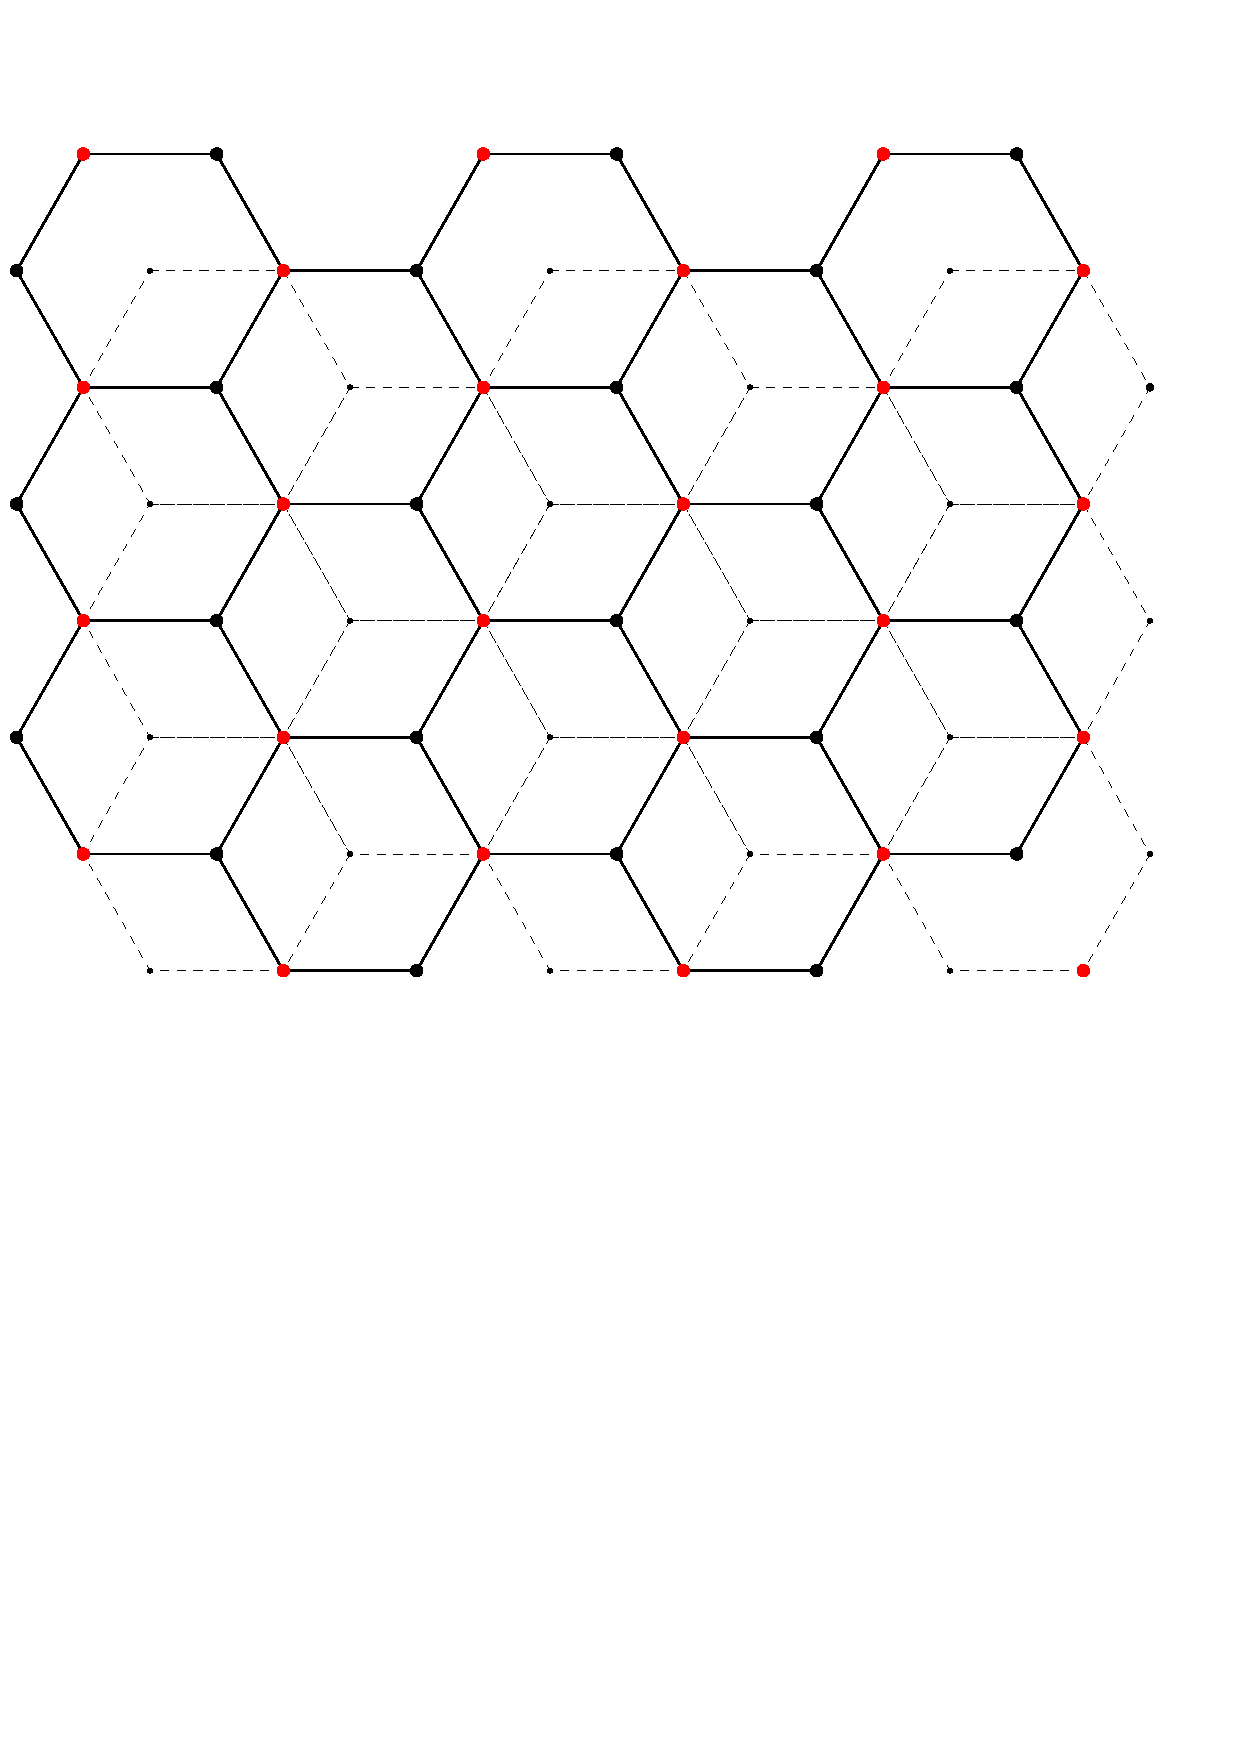
\includegraphics[width=0.6\textwidth]{grafiken/graphit.pdf}
  \caption{Schematische Darstellung der obersten zwei Ebenen eines Graphit-Kristalls. Die Kohlenstoffatome die in der oberen Ebene (fett) und der Unteren (gestrichelt) überlappen sind in rot markiert.}
  \label{fig:graphit}
\end{figure}
Graphit besteht aus planen Kohlenstoffebenen mit einer regelmäßigen hexagonalen Struktur.
Der Abstand der Kohlenstoffatome in einer solchen Ebene ist \SI{1,42}{\angstrom} \cite{colton}.
Diese Ebenen liegen unter einem Versatz übereinander, der das Zentrum eines Hexagons mit einem Kohlenstoffatom in der darunterliegenden Ebene zusammenfallen lässt (vgl. Abbildung \ref{fig:graphit}).
Aufgrund des Einflusses der überlappenden Kohlenstoffatome (in der Zeichnung rot) auf die elektronische Struktur an der Oberfläche, sind nur die nicht-überlappenden Atome bei der Bildgebung maßgeblich. Aus diesem Grund ist der Abstand der bei der Rastertunnelmikroskopie sichtbaren Kohlenstoffatome \SI{2,46}{\angstrom} ($=2 \cdot \SI{1,42}{\angstrom} \cdot \sin(60\si{\degree})$)

\subsection{Verwandte Rastermethoden}
\begin{itemize}
  \item \textbf{Rasterkraftmikroskopie:} Um nicht-leitende Oberflächen zu untersuchen ist die Rastertunnelmikroskopie ungeeignet.
  Stattdessen nutzt man die interatomaren Kräfte zwischen dem Objekt und einer Blattfeder mit dünner Spitze aus, um aus deren Auslenkung das Profil der Oberfläche zu bestimmen.
  Ähnlich zum RTM gibt es im Kontaktbetrieb des Rasterkraftmikroskops zwei typische Betriebsmodi:
  \begin{itemize}
  \item[--] konstante Kraft: Eine Rückkopplungsschleife zwischen Auslenkungsmessung und Höheneinstellung sorgt dafür, dass die Auslenkung und damit die Kraft konstant gehalten wird.
  So ist das Profil des Objektes gegeben durch die Blattfederhöhe.
  \item[--] konstante Höhe: Die Höheneinstellung bleibt unverändert und das Profil des Objektes ist gegeben durch die Auslenkung der Feder.
  \end{itemize}
  Es gibt noch weitere Betriebsmodi auf die hier nicht weiter eingegangen wird.
  \item \textbf{Rasterelektronenmikroskopie:} Ein gebündelter Elektronenstrahl wird über ein Objekt gerastert.
  Die dabei entstehenden gestreuten Elektronen, Sekundärelektronen, Bremsstrahlung etc. können über Detektoren eine Abbildung des Objekt reproduzieren.
\end{itemize}

\section{Versuchsdurchführung}

\section{Messdaten}

\section{Auswertung}

\section{Diskussion}

\section{Zusammenfassung}

% BIBLIOGRAPHIE

% Maximale Anzahl der Einträge in Klammer
% Zitieren mit \cite{lamport94}
\begin{thebibliography}{9}

% Beispiel
\bibitem{binning}
  G. Binning et al.,
  \emph{Surface Studies by Scanning Tunneling Microscopy},
  Phys. Rev. Lett. 49, 57 (1982).

\bibitem{colton}
  R. J. Colton, A. Engel, J. E. Frommer et al.,
  \emph{Procedures in Scanning Probe Microscopies},
  John Wiley 1998.
  
\end{thebibliography}

\end{document}
